% !TEX program = xelatex
\documentclass[tikz, crop, border = {2pt 2pt 2pt 2pt}]{standalone}

\usepackage{concmath-otf}
\usetikzlibrary{calc, angles, quotes, patterns, math}
\usetikzlibrary{decorations.pathreplacing, decorations.pathmorphing, calligraphy}

\usepackage{xcolor}
\definecolor{TheoremCol}{HTML}{C2D4FF}
\definecolor{TheoremColText}{HTML}{002469}
\definecolor{DefCol}{HTML}{DCF3CE}
\definecolor{DefColText}{HTML}{234210}
\definecolor{DefColAccent}{HTML}{A0E377}
\definecolor{AxiomCol}{HTML}{FFC2CA}
\definecolor{AxiomColText}{HTML}{4A0000}
\definecolor{AxiomColAccent}{HTML}{FF5C72}
\definecolor{LittleCol}{HTML}{FFC72B}
\definecolor{LittleColAccent}{HTML}{F7EDAD}

\begin{document}
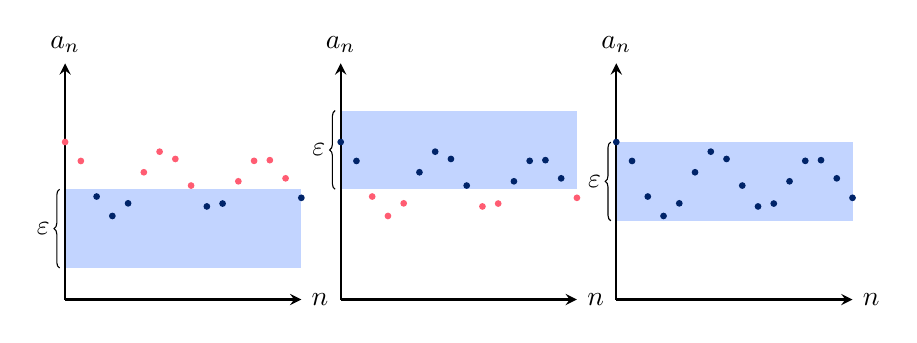
\begin{tikzpicture}
	\begin{scope}[shift = {(0, 0)}]
		\draw[thick, -stealth] (0, 0) -- (0, 3) node[above]{$a_n$};
		\draw[thick, -stealth] (0, 0) -- (3, 0) node[right]{$n$};
		\def\beg{0.4}
		\def\eps{1}
		\draw[decorate, decoration = {brace, amplitude = 2pt, raise = 2pt}] (0, \beg) -- node[left = 2pt]{$\varepsilon$} ++ (0, \eps);
		\fill[blend mode = multiply, TheoremCol] (0, \beg) rectangle ++ (3, \eps);
		\foreach \i [count = \xi] in {0, 0.2, 0.4, ..., 3} {
				\tikzmath{
					function seq(\i) {
							return {0.5 * cos(5 * \i r) * e^(-0.2 * \i) + 1.5};
						};
					\seq = seq(\i);
					if \seq - \beg >= \eps then {
							let \c = AxiomColAccent;
						} else {
							let \c = TheoremColText;
						};
				};
				\filldraw[color = \c] (\i, \seq) circle (1pt);
			}
	\end{scope}
	\begin{scope}[shift = {(3.5, 0)}]
		\draw[thick, -stealth] (0, 0) -- (0, 3) node[above]{$a_n$};
		\draw[thick, -stealth] (0, 0) -- (3, 0) node[right]{$n$};
		\def\beg{1.4}
		\def\eps{1}
		\draw[decorate, decoration = {brace, amplitude = 2pt, raise = 2pt}] (0, \beg) -- node[left = 2pt]{$\varepsilon$} ++ (0, \eps);
		\fill[blend mode = multiply, TheoremCol] (0, \beg) rectangle ++ (3, \eps);
		\foreach \i [count = \xi] in {0, 0.2, 0.4, ..., 3} {
				\tikzmath{
					function seq(\i) {
							return {0.5 * cos(5 * \i r) * e^(-0.2 * \i) + 1.5};
						};
					\seq = seq(\i);
					if (0 <= \seq - \beg) && (\seq - \beg <= \eps) then {
							let \c = TheoremColText;
						} else {
							let \c = AxiomColAccent;
						};
				}
				\filldraw[color = \c] (\i, \seq) circle (1pt);
			};
	\end{scope}
	\begin{scope}[shift = {(7, 0)}]
		\draw[thick, -stealth] (0, 0) -- (0, 3) node[above]{$a_n$};
		\draw[thick, -stealth] (0, 0) -- (3, 0) node[right]{$n$};
		\def\beg{1}
		\def\eps{1}
		\draw[decorate, decoration = {brace, amplitude = 2pt, raise = 2pt}] (0, \beg) -- node[left = 2pt]{$\varepsilon$} ++ (0, \eps);
		\fill[blend mode = multiply, TheoremCol] (0, \beg) rectangle ++ (3, \eps);
		\foreach \i [count = \xi] in {0, 0.2, 0.4, ..., 3} {
				\tikzmath{
					function seq(\i) {
							return {0.5 * cos(5 * \i r) * e^(-0.2 * \i) + 1.5};
						};
					\seq = seq(\i);
					if (0 <= \seq - \beg) && (\seq - \beg <= \eps) then {
							let \c = TheoremColText;
						} else {
							let \c = AxiomColAccent;
						};
				}
				\filldraw[color = \c] (\i, \seq) circle (1pt);
			};
	\end{scope}
\end{tikzpicture}
\end{document}
